\documentclass[UTF8,a4paper]{ctexart}
\usepackage[utf8]{inputenc}
\usepackage{amsmath}
\usepackage{pdfpages}
\usepackage{graphicx}
\usepackage{wrapfig}
\usepackage{listings}
\newcommand{\tabincell}[2]{\begin{tabular}{@{}#1@{}}#2\end{tabular}}
\title{实验一 单管放大电路仿真及实验}
\author{张蔚桐\ 2015011493\ 自55}
\begin {document}
\maketitle
\section{预习任务}
\subsection{电路放大原理}
\begin {wrapfigure}{r}{0pt}
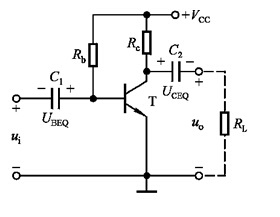
\includegraphics [width=40mm]{basic.jpg}
\caption{基本阻容耦合电路图}
\label{basic}
\end {wrapfigure}
以阻容耦合电路为例,如图\ref{basic}所示,集电极电源$V_{CC}$ 通过基极电阻$R_b$ 和集电极电阻$R_c$ 提供合适的$U_{be}$ 和$U_{ce}$,使晶体管处于放大区。为了保证放大电路正常工作,需要通过调整参数得到合适的静态工作点,保证输入信号在一定范围内时最终的信号不会失真。有交流小信号$u_i$ 作用时,交流量驼载在直流量上。输入信号通过容抗很小的电容加在发射结上,小电流经过晶体管放大后,在集电极产生放大的电流,通过$R_c$ 转换为电压变化,从而实现了对动态电压信号的放大。
\subsection{理论预估}
\begin {wrapfigure}{r}{0pt}
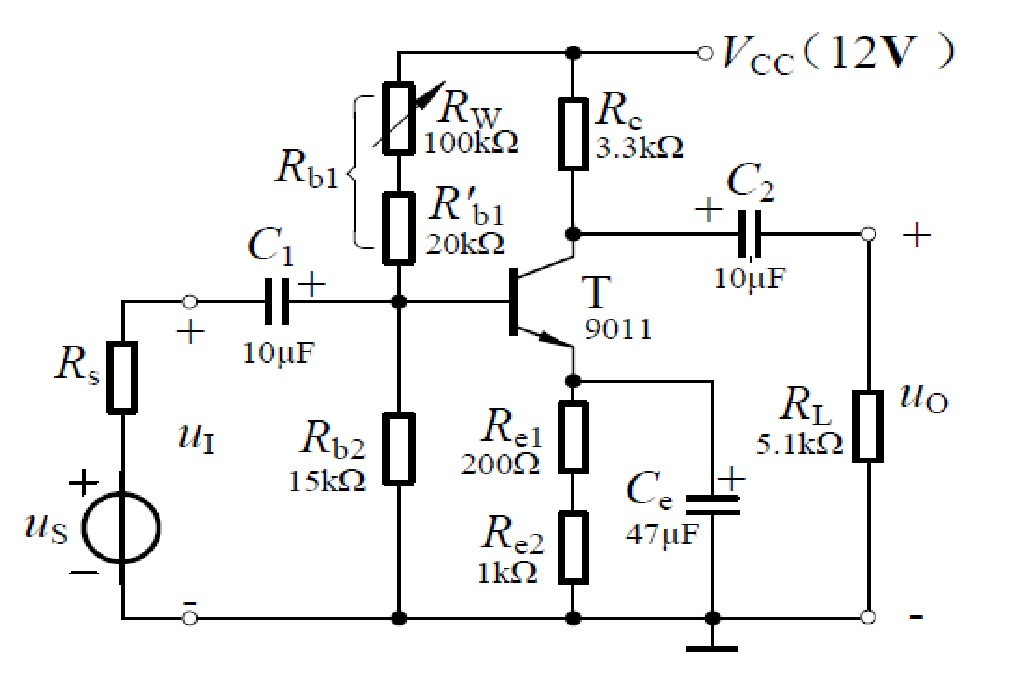
\includegraphics [width=60mm]{circuit.jpg}
\caption{单管共射放大电路}
\label{circuit}
\end {wrapfigure}
如图\ref{circuit}所示是实验用电路图,其中进行理论估算时取$r_{bb'}=100\Omega$于是可得$r_{be}=r_{bb'}+\frac{U_T}{I_{BQ}}\approx100\Omega+\frac{26\rm{mV}}{10\rm{\mu A}}\approx1\rm{k}$$\Omega$其中上式的各项参数按照经典值进行估计,$\beta$估计为100。上式仅为在数量级上的估计。

同样可以得到$R_i\approx10k\Omega,R_o\approx3.3k\Omega,\dot{A}=-\frac{\beta R_L'}{r_{be}}\approx-30$ 
\\ \\ \\ 

\section{EDA中对$\beta$的测量} 
\begin {wrapfigure}{r}{0pt}
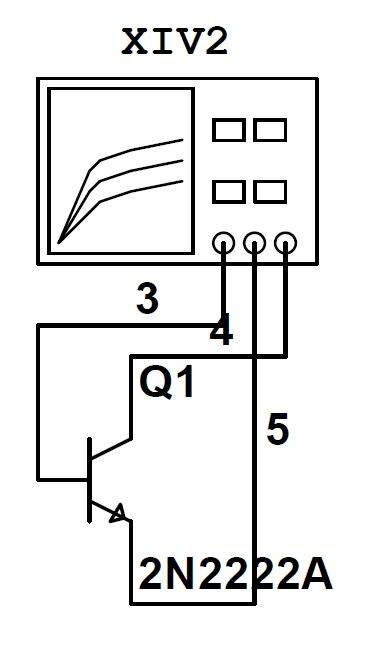
\includegraphics [width=40mm]{9.JPG}
\caption{晶体管$\beta$测试电路图}
\label{TCirc}
\end {wrapfigure}
采用如图\ref{TCirc}的电路进行测试,将晶体管按照IV测试仪的指示接入IV测试仪,将“Component”设置为“BJT NPN”,将$I_b$设置为$0\rm{A} -- 10\rm{\mu A} $,$U_{ce}$设置为0V~10V进行宽范围测试,得到图\ref{Tgeneral}所示的结果 
\begin {figure}
\centering
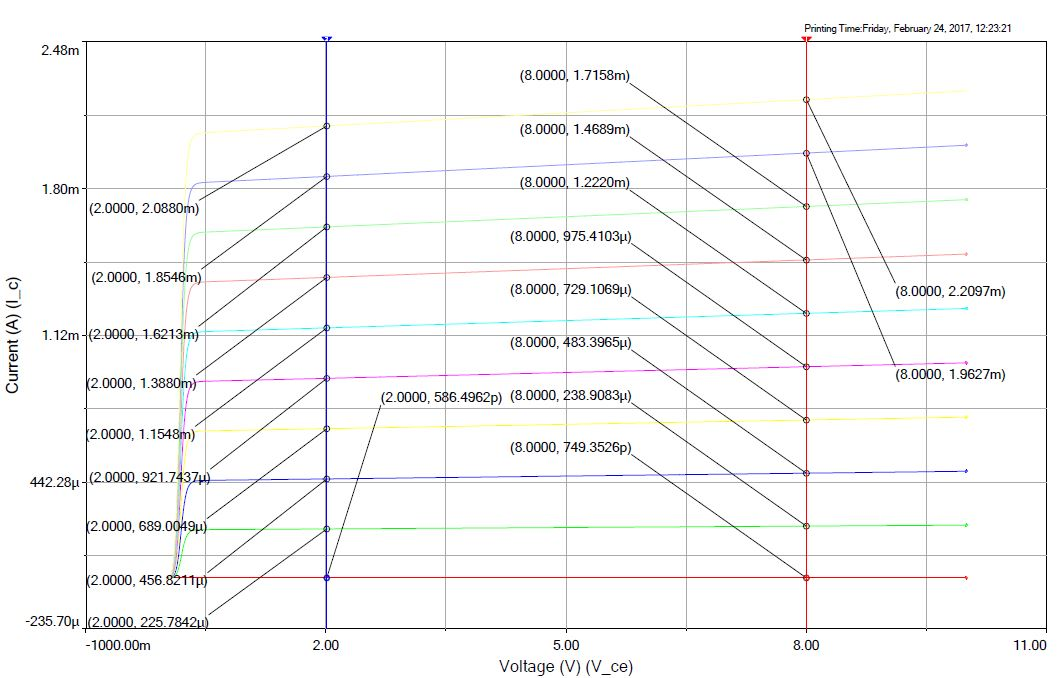
\includegraphics[width=\textwidth]{17.JPG}
\caption{晶体管输出特性}
\label{Tgeneral}
\end{figure}
在图\ref{Tgeneral}中标识了在$U_{ce}=2\rm{V}$和$U_{ce}=8\rm{V}$下,$I_c$随着$I_b$的变化情况,具体来说可以总结为下表
\\

\begin{tabular}{|c|c|c|}
\hline
\tabincell{c}{$I_b/\rm{\mu A}$}& \tabincell{c}{$I_c/\rm{mA}@U_{ce}=2\rm{V}$}& \tabincell{c}{$I_c/\rm{mA}@U_{ce}=8\rm{V}$}\\
\hline
0.00&0.0005&0.0007 \\
\hline
1.11&0.2258 &0.2389 \\
\hline
2.22&0.4568 &0.4834 \\
\hline
3.33&0.6890 &0.7291 \\
\hline
4.44&0.9217 &0.9754 \\
\hline
5.56&1.1549 &1.2220 \\
\hline
6.67&1.3880 &1.4689 \\
\hline
7.78&1.6213 &1.7158 \\
\hline
8.89&1.8546 &1.9627 \\
\hline
10&2.0880 &2.2097 \\
\hline
\end{tabular}
\\

于是可以对两种情况下的$I_c$和$I_b$做直线拟合得到
$$I_c=209.06I_b-5.2456(\rm{\mu A})@U_{ce}=2\rm{V},R^2=1,\beta=209.06$$
$$I_c=221.24I_b-5.5308(\rm{\mu A})@U_{ce}=8\rm{V},R^2=1,\beta=221.24$$

因此可以认为晶体管的$\beta=215$
\section{理论计算}

\end{document}